\chapter{Introduction}


% % Some applications of marine (Underwater and Aerial drones), suvryeing and wind trubine inspection
% Marine robotics has emerged as a transformative technology across diverse domains requiring underwater operations. For example, the offshore energy sector increasingly relies on underwater and aerial robots for routine inspection of wind turbines, identifying structural damage that could compromise operational integrity. Similarly, the oil and gas industry utilizes specialized underwater vehicles for pipeline inspection, identifying potential leaks or structural weaknesses over vast underwater networks. Marine robotics also plays a pivotal role in environmental monitoring, archaeological surveying, and defense applications including mine countermeasures and underwater surveillance.


% % Need for autonomy
% Autonomous operation is crucuial, as it reduces human risk and also reliability of these technologies.


% % PRoblems with marine robotics and why itr needs advanced control


% Despite significant advances, marine robotics faces unique challenges to be deployed fully autonomously for operations. There is a need for high precision control algorithms to can handle highly non linear, high digrees of freedom system, while excuting complex menauvers and trajectories.
% b) Handling uncertainties in oepration conditions such as currents, winds and s on 

% b) Generic Control Algorithms that would apply to the diverse nature of different robots






\section{Marine Robotics: Advancing Autonomy for Underwater and Aerial Applications}

Marine robotics encompasses a diverse array of platforms, including remotely operated vehicles (ROVs), autonomous underwater vehicles (AUVs), unmanned surface vehicles (USVs), and marine-focused unmanned aerial vehicles (UAVs or drones) (see Fig. \ref{fig:underwater_robotics_applications}). These systems are increasingly vital across multiple domains. In the energy sector, they can perform essential inspections of offshore wind turbines and subsea pipelines, detecting critical structural defects or leaks. Beyond industry, applications span environmental monitoring, archaeological surveying, scientific research, and defense operations like mine countermeasures and surveillance.


\begin{figure*}[!h]
    \centering
    % First Row
    \begin{subfigure}[b]{0.49\textwidth}
        \centering
        \includegraphics[width=\textwidth]{Phd_thesis/chapters/1.Introduction/figures/eelume.jpg}
        \caption{Kongsberg Eelume "snake" underwater robot \cite{kongsberg_eelume_nodate}.}
        \label{fig:subfig1}
    \end{subfigure}
    \hfill
    \begin{subfigure}[b]{0.49\textwidth}
        \centering
        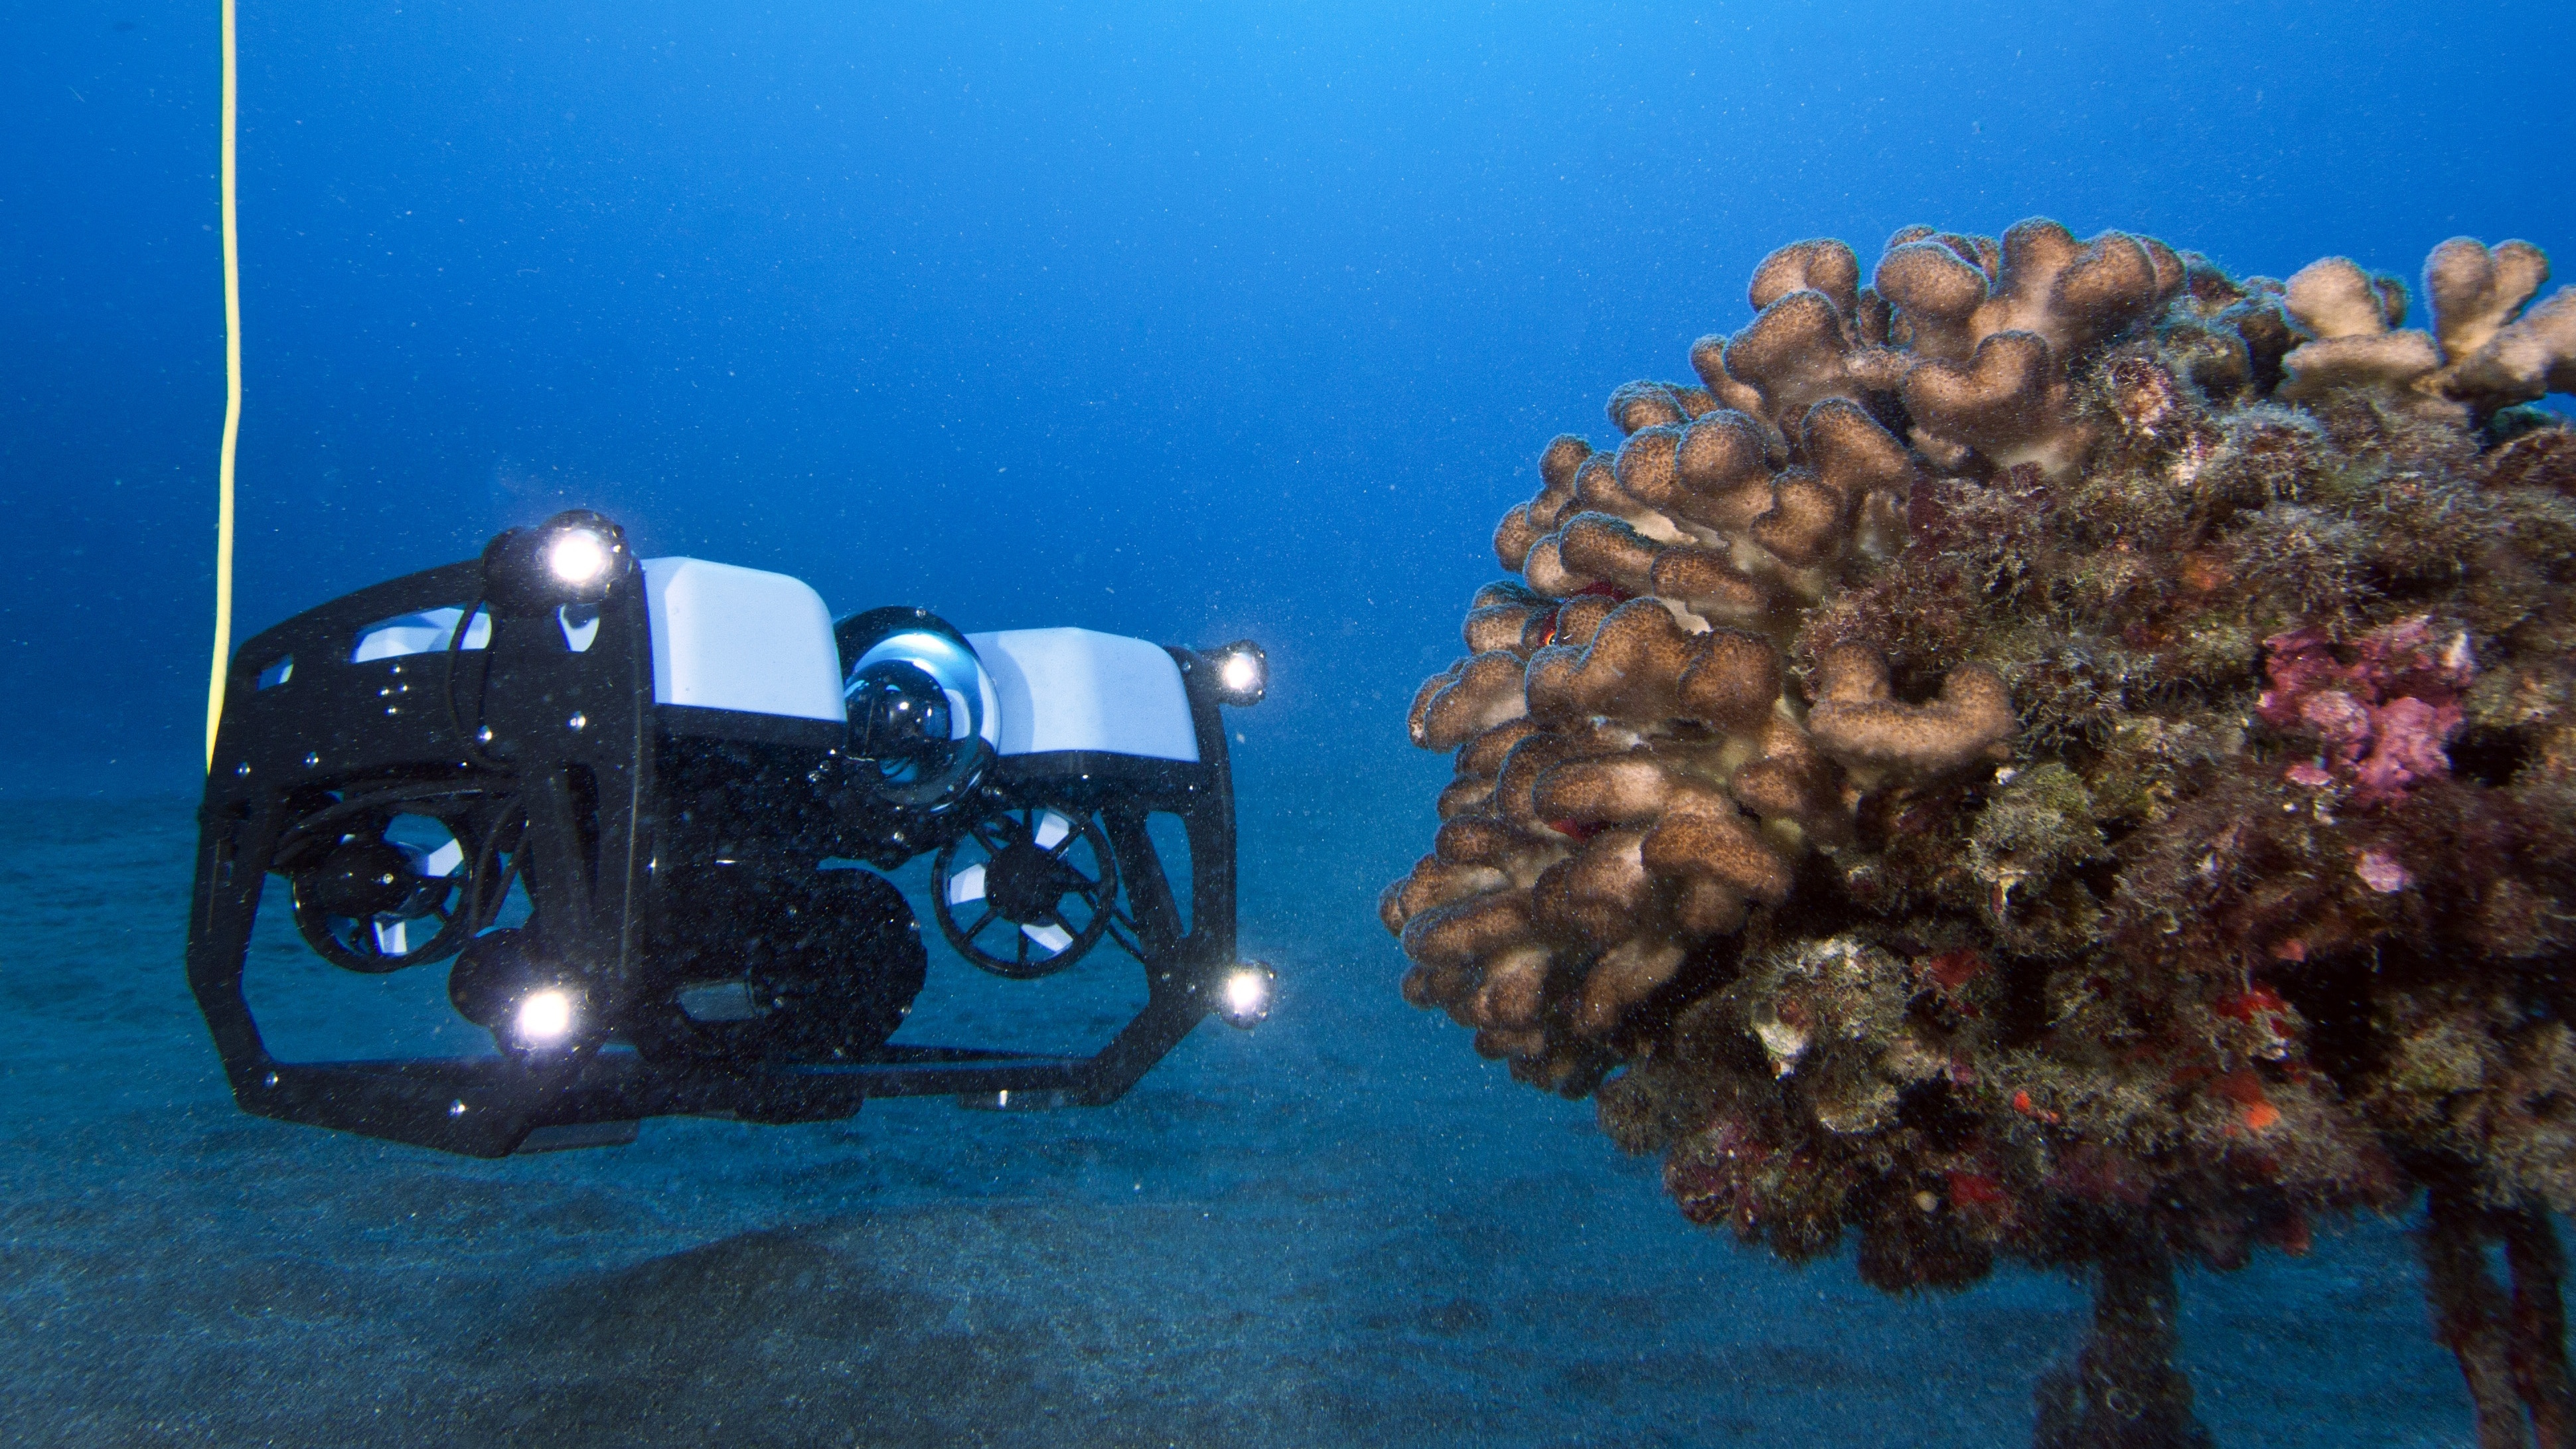
\includegraphics[width=\textwidth]{Phd_thesis/chapters/1.Introduction/figures/BlueROV2.jpg}
        \caption{BlueROV2 medium-sized tethered ROV \cite{bluerobotics_bluerov2_nodate}.}
        \label{fig:subfig2}
    \end{subfigure}
    
    \vspace{0.5cm} % Adjust vertical space between rows
    
    % Second Row
    \begin{subfigure}[b]{0.49\textwidth}
        \centering
        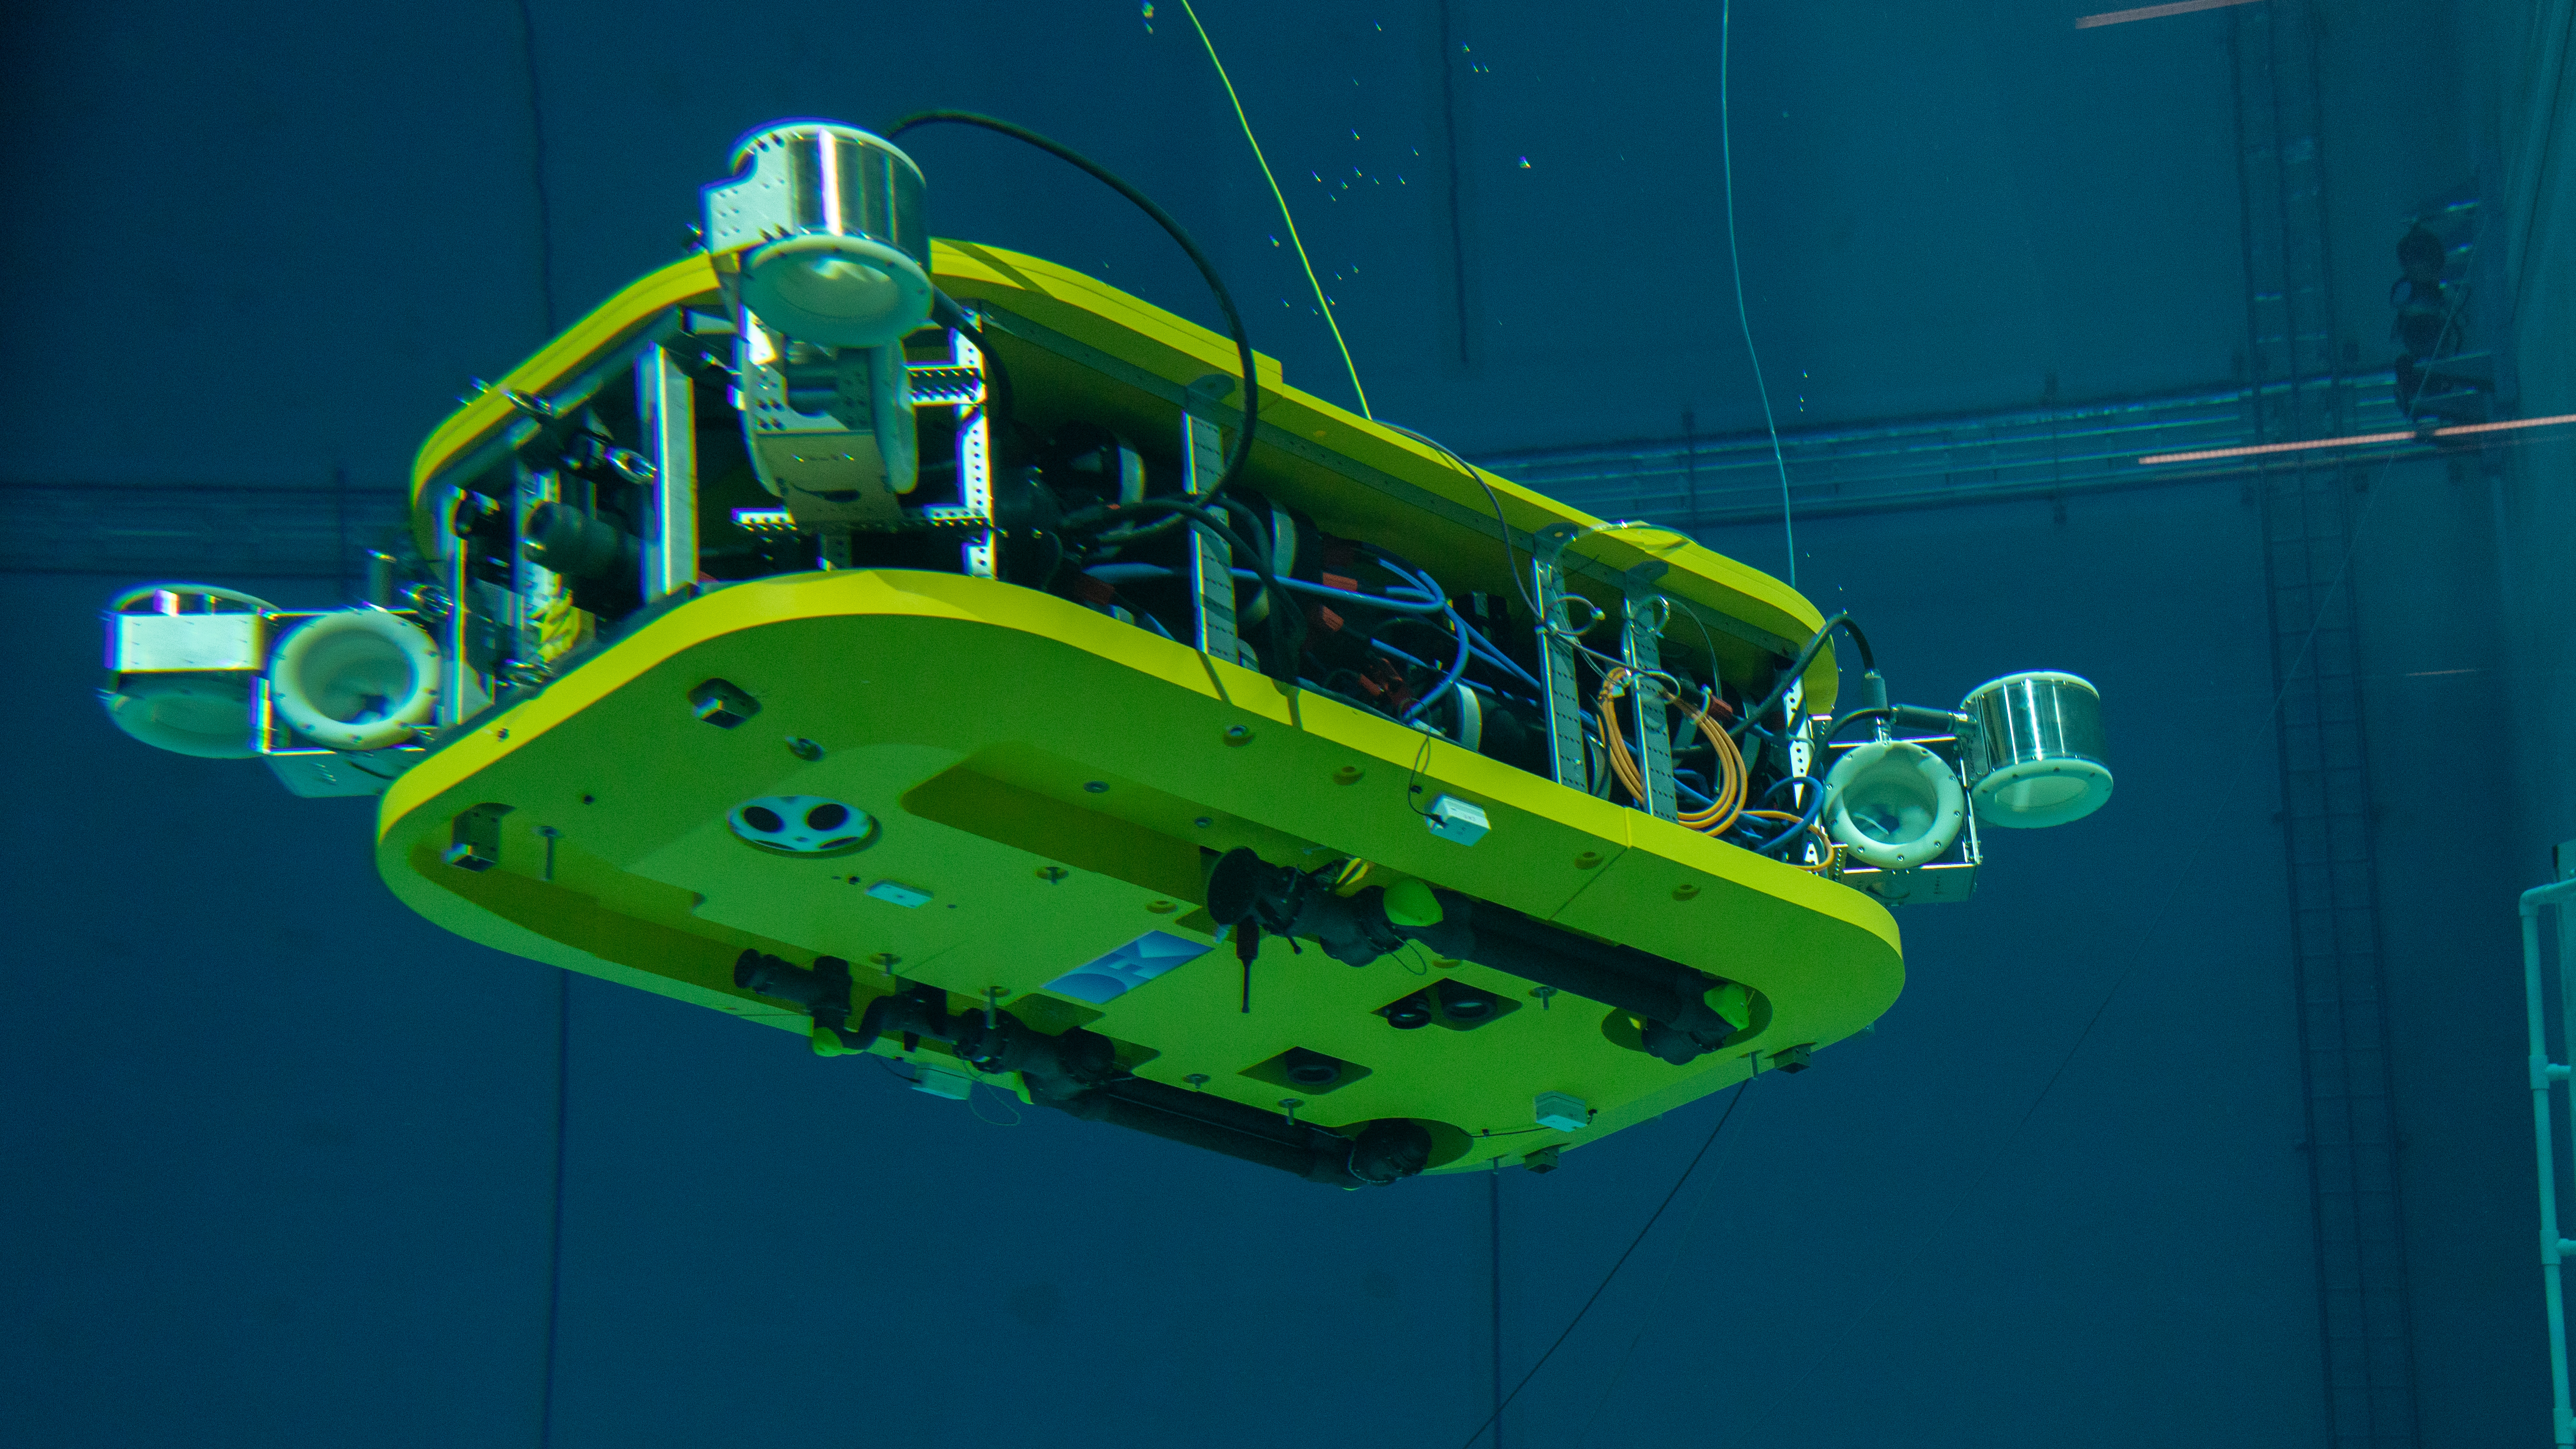
\includegraphics[width=\textwidth]{Phd_thesis/chapters/1.Introduction/figures/cuttlefish.jpg}
        \caption{DFKI Cuttlefish autonomous underwater vehicle \cite{christensen_cuttlefish_nodate}.}
        \label{fig:subfig3}
    \end{subfigure}
    \hfill
    \begin{subfigure}[b]{0.49\textwidth}
        \centering
        \includegraphics[width=\textwidth]{Phd_thesis/chapters/1.Introduction/figures/scanfish_towed.jpg}
        \caption{EIVA ScanFish Rocio remotely operated towed vehicle \cite{eiva_scanfish_nodate}.}
        \label{fig:subfig4}
    \end{subfigure}
    
    \caption{Showcase of the variety Marine Robotics Platforms.}
    \label{fig:underwater_robotics_applications}
\end{figure*}


Currently, many marine robotic tasks depend on remote control (teleoperation) or semi-autonomous functions, such as executing pre-programmed paths or simple line-following maneuvers. While effective for specific, well-defined tasks, these modes often necessitate skilled human pilots and constant supervision, limiting mission duration, complexity, and operational range.

The drive towards fully autonomous marine systems stems from the need to enhance operational safety, increase mission efficiency and capability, and reduce operational costs. By minimizing direct human intervention, autonomy mitigates the risk of human error, enables longer and more complex missions in challenging environments, and ultimately lowers operational expenses.


% --- Challenges to Autonomy ---
Achieving reliable underwater autonomy, however, requires overcoming fundamental challenges inherent to the complex and dynamic marine environment. Key among these are:

\begin{itemize}
    \item \textbf{Robustness to Disturbances:} Marine robots must maintain stable operation and achieve mission objectives despite unpredictable environmental factors. For instance, an \ac{AUV} mapping the seafloor needs to adhere to its planned trajectory even when strong, unmodelled currents attempt to push it off course.
    \item \textbf{Generalizability Across Diverse Missions and Platforms:} Control strategies should be adaptable to various marine vehicle types (e.g., \acp{AUV}, \acp{ROV}) and a wide range of tasks (e.g., inspection, survey, manipulation) without requiring complete redesign for each specific case.
    \item \textbf{Execution of Complex Maneuvers:} True autonomy demands the capability to perform intricate and precise tasks, such as docking with an underwater charging station, coordinating multi-robot search patterns while avoiding collisions, or navigating complex subsea structures for close inspection.
\end{itemize}

% The drive towards fully autonomous marine systems stems from the need to enhance operational safety, efficiency, capability, and reduce operational costs. By minimizing human intervention, autonomy lowers error risks and enables longer, and complex missions improving effectiveness and lowering expenses.


% Achieving reliable underwater autonomy requires overcoming some fundamental challenges, and importantly, these include:

% \textbf{Robustness in the Face of Disturbances:} Marine robots must maintain operation despite unpredictable environmental factors. For example, an \ac{AUV} mapping the seafloor needs to stay on its planned path even when strong currents try to push it off course.

% \textbf{Generalizability Across Diverse Missions and Platforms:} Control systems should be adaptable to various marine vehicles and tasks without significant redesign. For instance, the core control logic for an ROV inspecting a pipeline should be transferable, with adjustments, to a  conducting oceanographic surveys.

% \textbf{Execution of Complex Maneuvers:} Autonomous systems must be capable of performing intricate tasks. This could involve an \ac{AUV} precisely docking with an underwater charging station or a group of UAVs coordinating to perform a complex search pattern while avoiding collisions.

% These challenges underscore the value of model-based strategies like \ac{MPC}, whose predictive capabilities and constraint handling directly address marine autonomy's core requirements. 














